\documentclass[12pt,a4paper]{article}

\usepackage[T1]{fontenc}
\usepackage[utf8]{inputenc}
\usepackage[magyar]{babel}
\usepackage{lmodern}
\usepackage{geometry}
\usepackage{graphicx}
\usepackage{float}
\usepackage{booktabs}
\geometry{margin=2.5cm}

\begin{document}

\begin{titlepage}
    \centering
    
    {\scshape\LARGE Miskolci Egyetem \par}
    \vspace{0.5cm}
    {\scshape\Large Gépészmérnöki és Informatikai Kar \par}
    \vspace{0.5cm}
    {\scshape\large Informatikai Intézet \par}
    
    \vspace{2.5cm}
    
    {\Huge\bfseries Conway-féle Game of Life párhuzamos megvalósítása OpenCL segítségével\par}
    
    \vspace{2cm}
    
    {\Large Féléves feladat\par}
    
    \vfill
    
    \begin{flushleft}
        \large
        \textbf{Szerző:} Gál Olivér István \\
        \textbf{Neptun-kód:} ISXBF3
    \end{flushleft}
    
    \vspace{1cm}
    
    \begin{flushright}
        \large
        Miskolc \\
        2026
    \end{flushright}
    
\end{titlepage}

\tableofcontents
\newpage

\section{Bevezetés}

A Conway-féle Game of Life egy klasszikus sejtautomata, amely egyszerű szabályok alapján modellezi egy kétdimenziós rács celláinak fejlődését. Minden cella két állapot valamelyikében lehet: élő vagy halott. Az egymást követő generációk során az adott cella új állapota a szomszédos cellák aktuális állapotától függ. Bár a szabályrendszer egyszerű, a rendszer viselkedése rendkívül változatos és összetett lehet.

A Game of Life különösen alkalmas párhuzamos feldolgozás vizsgálatára, mivel egy adott generációban a cellák új állapota egymástól függetlenül, az előző állapot alapján számítható ki. Ez lehetővé teszi, hogy a rács különböző részeit egyszerre, párhuzamosan dolgozzuk fel. Emiatt a feladat jól szemlélteti a GPU-alapú számítás és az adatpárhuzamosság előnyeit.

A beadandó célja egy OpenCL-alapú Game of Life megvalósítás elkészítése és teljesítményének vizsgálata volt. A megoldás során két különböző kernelváltozat készült: egy egyszerű, naiv implementáció, valamint egy optimalizált, \emph{tiled} megközelítés, amely lokális memóriát használ. A fejlesztés során a hangsúly nemcsak a működő program elkészítésén, hanem a különböző megoldások teljesítményének összehasonlításán is volt.

A program paraméterezhető módon kezeli a rács méretét, az iterációk számát, a \emph{work-group} méretet, valamint a peremkezelés módját is. A futások eredményei CSV formátumban menthetők, és grafikonok segítségével is elemezhetők. A mérések célja annak bemutatása volt, hogy a lokális memória használata és a megfelelő \emph{work-group} méret hogyan befolyásolja a futási időt és a teljesítményt.

\section{A feladat ismertetése}

A Game of Life egy kétdimenziós rácson működő sejtautomata. A rács minden eleme egy cellát reprezentál, amely kétféle állapotot vehet fel: élő vagy halott. Az állapotok változása diszkrét időlépésekben, úgynevezett iterációkban történik. Minden új generáció kiszámítása az előző generáció teljes állapota alapján történik.

Egy cella állapotát a nyolc közvetlen szomszédja befolyásolja: a vízszintes, függőleges és átlós irányban közvetlenül mellette lévő cellák. Az állapotfrissítés szabályai a következők:

\begin{itemize}
    \item ha egy élő cellának kettő vagy három élő szomszédja van, életben marad,
    \item ha egy élő cellának kettőnél kevesebb vagy háromnál több élő szomszédja van, elpusztul,
    \item ha egy halott cellának pontosan három élő szomszédja van, élővé válik.
\end{itemize}

A feladat során egy olyan OpenCL-alapú alkalmazás készült, amely képes a Game of Life több iteráción keresztüli futtatására GPU-n vagy OpenCL-t támogató eszközön. A rács kezdeti állapota véletlenszerűen generálódik, majd az alkalmazás a megadott számú iteráción keresztül számolja a következő generációkat.

A megvalósítás kétféle peremkezelést is támogat. Az első esetben a rácson kívüli cellák halottnak számítanak (\texttt{wrap=0}), tehát a széleken a szomszédsági vizsgálat csak a rácson belüli elemekre korlátozódik. A második esetben toroidális peremkezelést használunk (\texttt{wrap=1}), ahol a rács szélei összeérnek: a bal szél a jobb széllal, a felső szél az alsóval. Ez azt jelenti, hogy a szélső cellák szomszédai a túloldalról is számításba kerülnek.

A cél nem csupán a helyes működés biztosítása volt, hanem annak vizsgálata is, hogyan teljesít különböző OpenCL-megoldásokkal ugyanaz a feladat. Ennek érdekében egy egyszerű, közvetlen memóriaműveletekre épülő naiv kernel, valamint egy lokális memóriát használó, optimalizált \emph{tiled} kernel is elkészült.

\section{A megvalósítás célja és fő irányai}

A projekt célja egy olyan OpenCL-alapú Game of Life alkalmazás elkészítése volt, amely képes nagyméretű rácsok több iteráción keresztüli feldolgozására, miközben lehetőséget ad a különböző megoldások teljesítményének összehasonlítására is. A fejlesztés során fontos szempont volt, hogy a program ne csak működőképes legyen, hanem mérhető és elemezhető módon is támogassa a teljesítményvizsgálatot.

A megvalósítás során két kernelváltozat készült. Az első egy egyszerű, naiv megoldás, ahol minden \emph{work-item} közvetlenül a globális memóriából olvassa ki a szükséges szomszédos cellákat. Ez a megközelítés jól áttekinthető és könnyen implementálható, ugyanakkor nagy számú memóriaelérést igényel. A második változat egy optimalizált, \emph{tiled} megoldás, amely a \emph{work-group} által feldolgozott rácsrészletet lokális memóriába tölti be, így csökkenti a globális memóriaelérések számát.

A program parancssori paraméterekkel vezérelhető, így a rácsméret, az iterációk száma, a peremkezelési mód, a kernel típusa, valamint a \emph{work-group} méret is egyszerűen változtatható. Ez lehetővé teszi különböző konfigurációk vizsgálatát ugyanazon programon belül.

A mérési folyamat támogatására a program képes a host--device másolási idő, a kernel futási ideje, a device--host másolási idő, valamint ezek összegzett, OpenCL eseményprofilozással mért végrehajtási idejének mérésére és CSV fájlba mentésére. A kapott eredményekből grafikonok készíthetők, amelyek jól szemléltetik az egyes implementációk közötti különbségeket.

\section{A program felépítése}

A program felépítése moduláris, a host oldali vezérlés és a kerneloldali számítás jól elkülönül egymástól. A host oldali logika a \texttt{main.c} fájlban található, míg a számítási magot a különálló OpenCL kernel fájlok valósítják meg. A projekt két kernelváltozatot tartalmaz: egy egyszerű, közvetlen memóriaelérésre épülő \texttt{gol\_naive.cl} fájlt, valamint egy lokális memóriát használó, optimalizált \texttt{gol\_tiled.cl} megoldást.

A \texttt{main.c} feladata a program teljes végrehajtásának vezérlése. Ez magában foglalja a parancssori argumentumok feldolgozását, a kezdeti rács létrehozását, az OpenCL platform és eszköz kiválasztását, a kontextus és a parancssor létrehozását, a kernel forrásfájl betöltését és lefordítását, továbbá a szükséges pufferek lefoglalását. A host oldal emellett gondoskodik a kernelparaméterek beállításáról, a mérések végrehajtásáról, valamint az eredmények kiírásáról is.

A kernelbetöltés külön segédfüggvényen keresztül történik. A program a kiválasztott futtatási mód alapján dönti el, hogy a naiv vagy a \emph{tiled} kernel forrását töltse be. Ezt követően a kernel forrásából OpenCL program objektum jön létre, majd megtörténik annak fordítása és a megfelelő kernel példányosítása. A megoldás előnye, hogy ugyanaz a host oldali kód több kernelváltozatot is képes kezelni.

A program több parancssori paraméter segítségével vezérelhető. Beállítható a rács sor- és oszlopszáma, az iterációk száma, a véletlenszám-generátor magja, a peremkezelés módja, a kiválasztott kernel típusa, valamint a \emph{work-group} méretét meghatározó \texttt{lx} és \texttt{ly} érték. Emellett a program támogatja a többszöri ismételt futtatást és a bemelegítő futtatásokat is, ami pontosabb mérési eredmények elérését teszi lehetővé.

A mérési folyamat során a program külön kezeli a host--device adatmásolás, a kernel futás és a device--host visszaolvasás idejét. A futási idők méréséhez eseményalapú OpenCL profilozás tartozik minden fontosabb művelethez. Az így nyert adatok alapján külön meghatározható a kernel teljes futási ideje, valamint a host--device másolás, a kernel futás és a device--host visszaolvasás összegzett, profilozott végrehajtási ideje is. A program képes az eredményeket CSV formátumban menteni, így azok később egyszerűen feldolgozhatók grafikonrajzoló szkriptekkel vagy táblázatkezelővel.

A teljes végrehajtás menete tehát röviden a következő: a host oldal előállítja a kezdeti rácsot, kiválasztja és inicializálja az OpenCL környezetet, betölti a megfelelő kernelt, lefuttatja a megadott számú iterációt, majd kiolvassa és eltárolja a mérési eredményeket. Ez az elrendezés jól áttekinthető, és megfelelő alapot biztosít az implementációk közötti teljesítmény-összehasonlításhoz.

\section{A naiv OpenCL megoldás}

A naiv OpenCL megoldás célja a Game of Life szabályainak közvetlen, egyszerű és jól követhető implementálása volt. Ebben a megközelítésben minden \emph{work-item} egyetlen cella következő állapotának kiszámításáért felelős. A kernel a globális azonosítók alapján meghatározza, hogy az adott végrehajtási példány a rács melyik celláját dolgozza fel, majd kiolvassa annak nyolc szomszédját, összeszámolja az élő szomszédokat, és ezek alapján eldönti a cella következő állapotát.

A megoldás előnye, hogy logikailag nagyon közel áll a probléma eredeti definíciójához. Minden cella új állapota kizárólag az előző generáció adatai alapján számítódik ki, ezért az egyes cellák feldolgozása egymástól függetlenül történhet. Ez a fajta adatpárhuzamosság teszi lehetővé, hogy a Game of Life jól illeszkedjen az OpenCL végrehajtási modelljéhez.

A naiv kernel működése során azonban minden egyes cella feldolgozásakor több globális memóriaelérés történik. Egyetlen új cellaállapot kiszámításához ki kell olvasni a középponti cellát és annak szomszédságát is, ami jelentős mennyiségű memória-hozzáférést eredményez. Mivel a szomszédos cellák adatai sok esetben több \emph{work-item} számára is azonosak, a globális memóriaolvasások között jelentős átfedés alakul ki. Ez a megközelítés tehát funkcionálisan egyszerű, de teljesítmény szempontjából nem optimális.

A kernel támogatja a kétféle peremkezelési módot is. \texttt{wrap=0} esetén a rácson kívüli cellák halottnak számítanak, míg \texttt{wrap=1} esetén a koordináták körbefordulnak, így a rács toroidális módon viselkedik. Ez a funkcionalitás a naiv megoldásban közvetlenül a szomszédcellák koordinátáinak kezelésén keresztül jelenik meg.

A naiv megoldás fontos szerepet tölt be a projektben, mert jól értelmezhető referenciaimplementációt biztosít. Segítségével összehasonlíthatóvá válik, hogy a később bevezetett optimalizációk, különösen a lokális memória használata, mekkora teljesítményjavulást eredményeznek. Emiatt a naiv kernel nemcsak önálló megoldásként, hanem viszonyítási alapként is lényeges része a beadandónak.

\section{A tiled OpenCL megoldás}

A \emph{tiled} OpenCL megoldás a naiv verzió továbbfejlesztett, optimalizált változata. A fő cél az volt, hogy csökkenjen a globális memóriaelérések száma, mivel a naiv megközelítésben ugyanazon szomszédos cellák adatait több \emph{work-item} is újra és újra beolvassa. Ennek elkerülésére a \emph{tiled} megoldás a rács egy részletét a globális memóriából a gyorsabban elérhető lokális memóriába tölti, majd a számításokat ezen a lokális másolaton végzi el.

A megoldás alapegysége egy \emph{tile}, vagyis a rács egy olyan részlete, amelyet egy \emph{work-group} dolgoz fel. A lokális memóriába nemcsak a ténylegesen feldolgozandó cellák kerülnek be, hanem egy egycellás vastagságú úgynevezett \emph{halo} réteg is. Erre azért van szükség, mert a szélső cellák következő állapotának meghatározásához a tile-on kívüli közvetlen szomszédokat is figyelembe kell venni. A halo tehát biztosítja, hogy a work-group minden szükséges szomszédos adatot elérjen anélkül, hogy a számítás közben ismételten a globális memóriához kellene fordulnia.

A lokális memória feltöltése együttműködő módon történik. A \emph{work-itemek} nemcsak a saját középponti cellájukat töltik be, hanem a tile szélein és sarkaiban elhelyezkedő szálak a halo-elemek beolvasásában is részt vesznek. Miután minden szükséges adat bekerült a lokális memóriába, egy szinkronizációs pont biztosítja, hogy a \emph{work-group} összes tagja csak ezután kezdje meg a tényleges számítást.

A \emph{tiled} megoldás előnye, hogy a szomszédsági vizsgálat során a legtöbb adat már a lokális memóriából érhető el. Ez jóval kisebb késleltetésű hozzáférést jelent, mint a globális memória használata, így csökkenthető a memóriaelérések költsége és javítható a teljes futási idő. Különösen nagyobb rácsméretek és sok iteráció esetén válik jól láthatóvá ez az előny.

A megoldás támogatja a rugalmas \emph{work-group} méretet is, így a host oldalról megadható, hogy mekkora lokális csoportokkal történjen a végrehajtás. Ez lehetővé teszi a különböző konfigurációk teljesítményvizsgálatát. A mérések alapján a \emph{tiled} megközelítés egyértelműen gyorsabbnak bizonyult a naiv változatnál, ami igazolja, hogy a lokális memória használata hatékony optimalizáció a feladat esetén.

\section{Mérési környezet és módszertan}

A teljesítménymérések célja annak vizsgálata volt, hogy a Game of Life OpenCL-alapú megvalósításában a különböző kernelváltozatok és \emph{work-group} beállítások milyen teljesítményt nyújtanak eltérő rácsméretek mellett. A vizsgálat középpontjában a naiv és a lokális memóriát használó \emph{tiled} megoldás összehasonlítása állt.

A fő mérési sorozatban négy különböző rácsméretet vizsgáltam: \texttt{512x512}, \texttt{1024x1024}, \texttt{2048x2048} és \texttt{4096x4096}. Az iterációk számát a rácsméret függvényében választottam meg, hogy minden esetben elegendő mennyiségű számítás történjen, ugyanakkor a futtatási idő még kezelhető maradjon. A használt beállítások rendre \texttt{2000}, \texttt{1000}, \texttt{500} és \texttt{250} iterációk voltak.

A mérések során három konfigurációt hasonlítottam össze. Referenciaként a naiv implementáció \texttt{16x16} méretű \emph{work-group} beállítással szerepelt. Emellett két \emph{tiled} konfigurációt vizsgáltam: \texttt{8x8} és \texttt{16x16} méretű \emph{work-groupokat}. Ezzel lehetővé vált annak elemzése, hogy nemcsak a lokális memória használata, hanem a csoportméret megválasztása is hogyan hat a teljesítményre.

A fő mérési sorozatban a peremkezelési mód \texttt{wrap=0} volt, vagyis a rácson kívüli cellák halottnak számítottak. Ezt egységes referencia-beállításként választottam, hogy a különböző implementációk összehasonlítása közvetlenül és egyszerűen értelmezhető legyen. Kiegészítő vizsgálatként külön mérési sorozat készült a \texttt{wrap=0} és \texttt{wrap=1} beállítások összehasonlítására is \texttt{1024x1024} és \texttt{2048x2048} rácsméretek mellett.

A mérési eredmények megbízhatóságának növelése érdekében minden konfiguráció esetén egy bemelegítő futtatást (\texttt{warmup=1}) és öt ismétlést (\texttt{repeat=5}) alkalmaztam. A dokumentációban szereplő eredmények az ismételt futtatások átlagértékei. Ez csökkenti annak valószínűségét, hogy egyetlen futás esetleges eltérése torzítsa az eredményeket.

A mérések automatizálására külön batch fájlok készültek. A fő mérési sorozatot a \texttt{bench.bat} hajtotta végre, amely a négy vizsgált rácsméretre lefuttatta a naiv \texttt{16x16}, valamint a \emph{tiled} \texttt{8x8} és \texttt{16x16} konfigurációkat. A peremkezelés hatásának vizsgálatát a \texttt{bench\_wrap.bat} végezte, amely két rácsméreten hasonlította össze a \texttt{wrap=0} és \texttt{wrap=1} beállításokat a naiv, illetve a \emph{tiled 16x16} konfigurációk esetén.

A program OpenCL eseményalapú profilozással külön mérte a host--device adatmásolás, a kernel futás és a device--host visszaolvasás idejét. Az értékelés során a fő hangsúlyt a kernel futási idejére helyeztem, mivel az implementációk közötti különbség elsősorban itt jelenik meg. A kernelidőből iterációnkénti átlagidőt számítottam, továbbá meghatároztam a \emph{tiled} megoldások gyorsulását a naiv implementációhoz képest.

A mérési eredmények feldolgozására Python szkriptek készültek. A \texttt{plot\_results.py} a fő mérési sorozat eredményeiből három grafikont állított elő: a kernelidő / iteráció diagramot, a naiv verzióhoz viszonyított gyorsulást, valamint az összegzett profilozott végrehajtási idő alakulását. A \texttt{plot\_wrap\_results.py} külön ábrán szemléltette a peremkezelés módjának hatását a kernel futási idejére.

\begin{figure}[H]
    \centering
    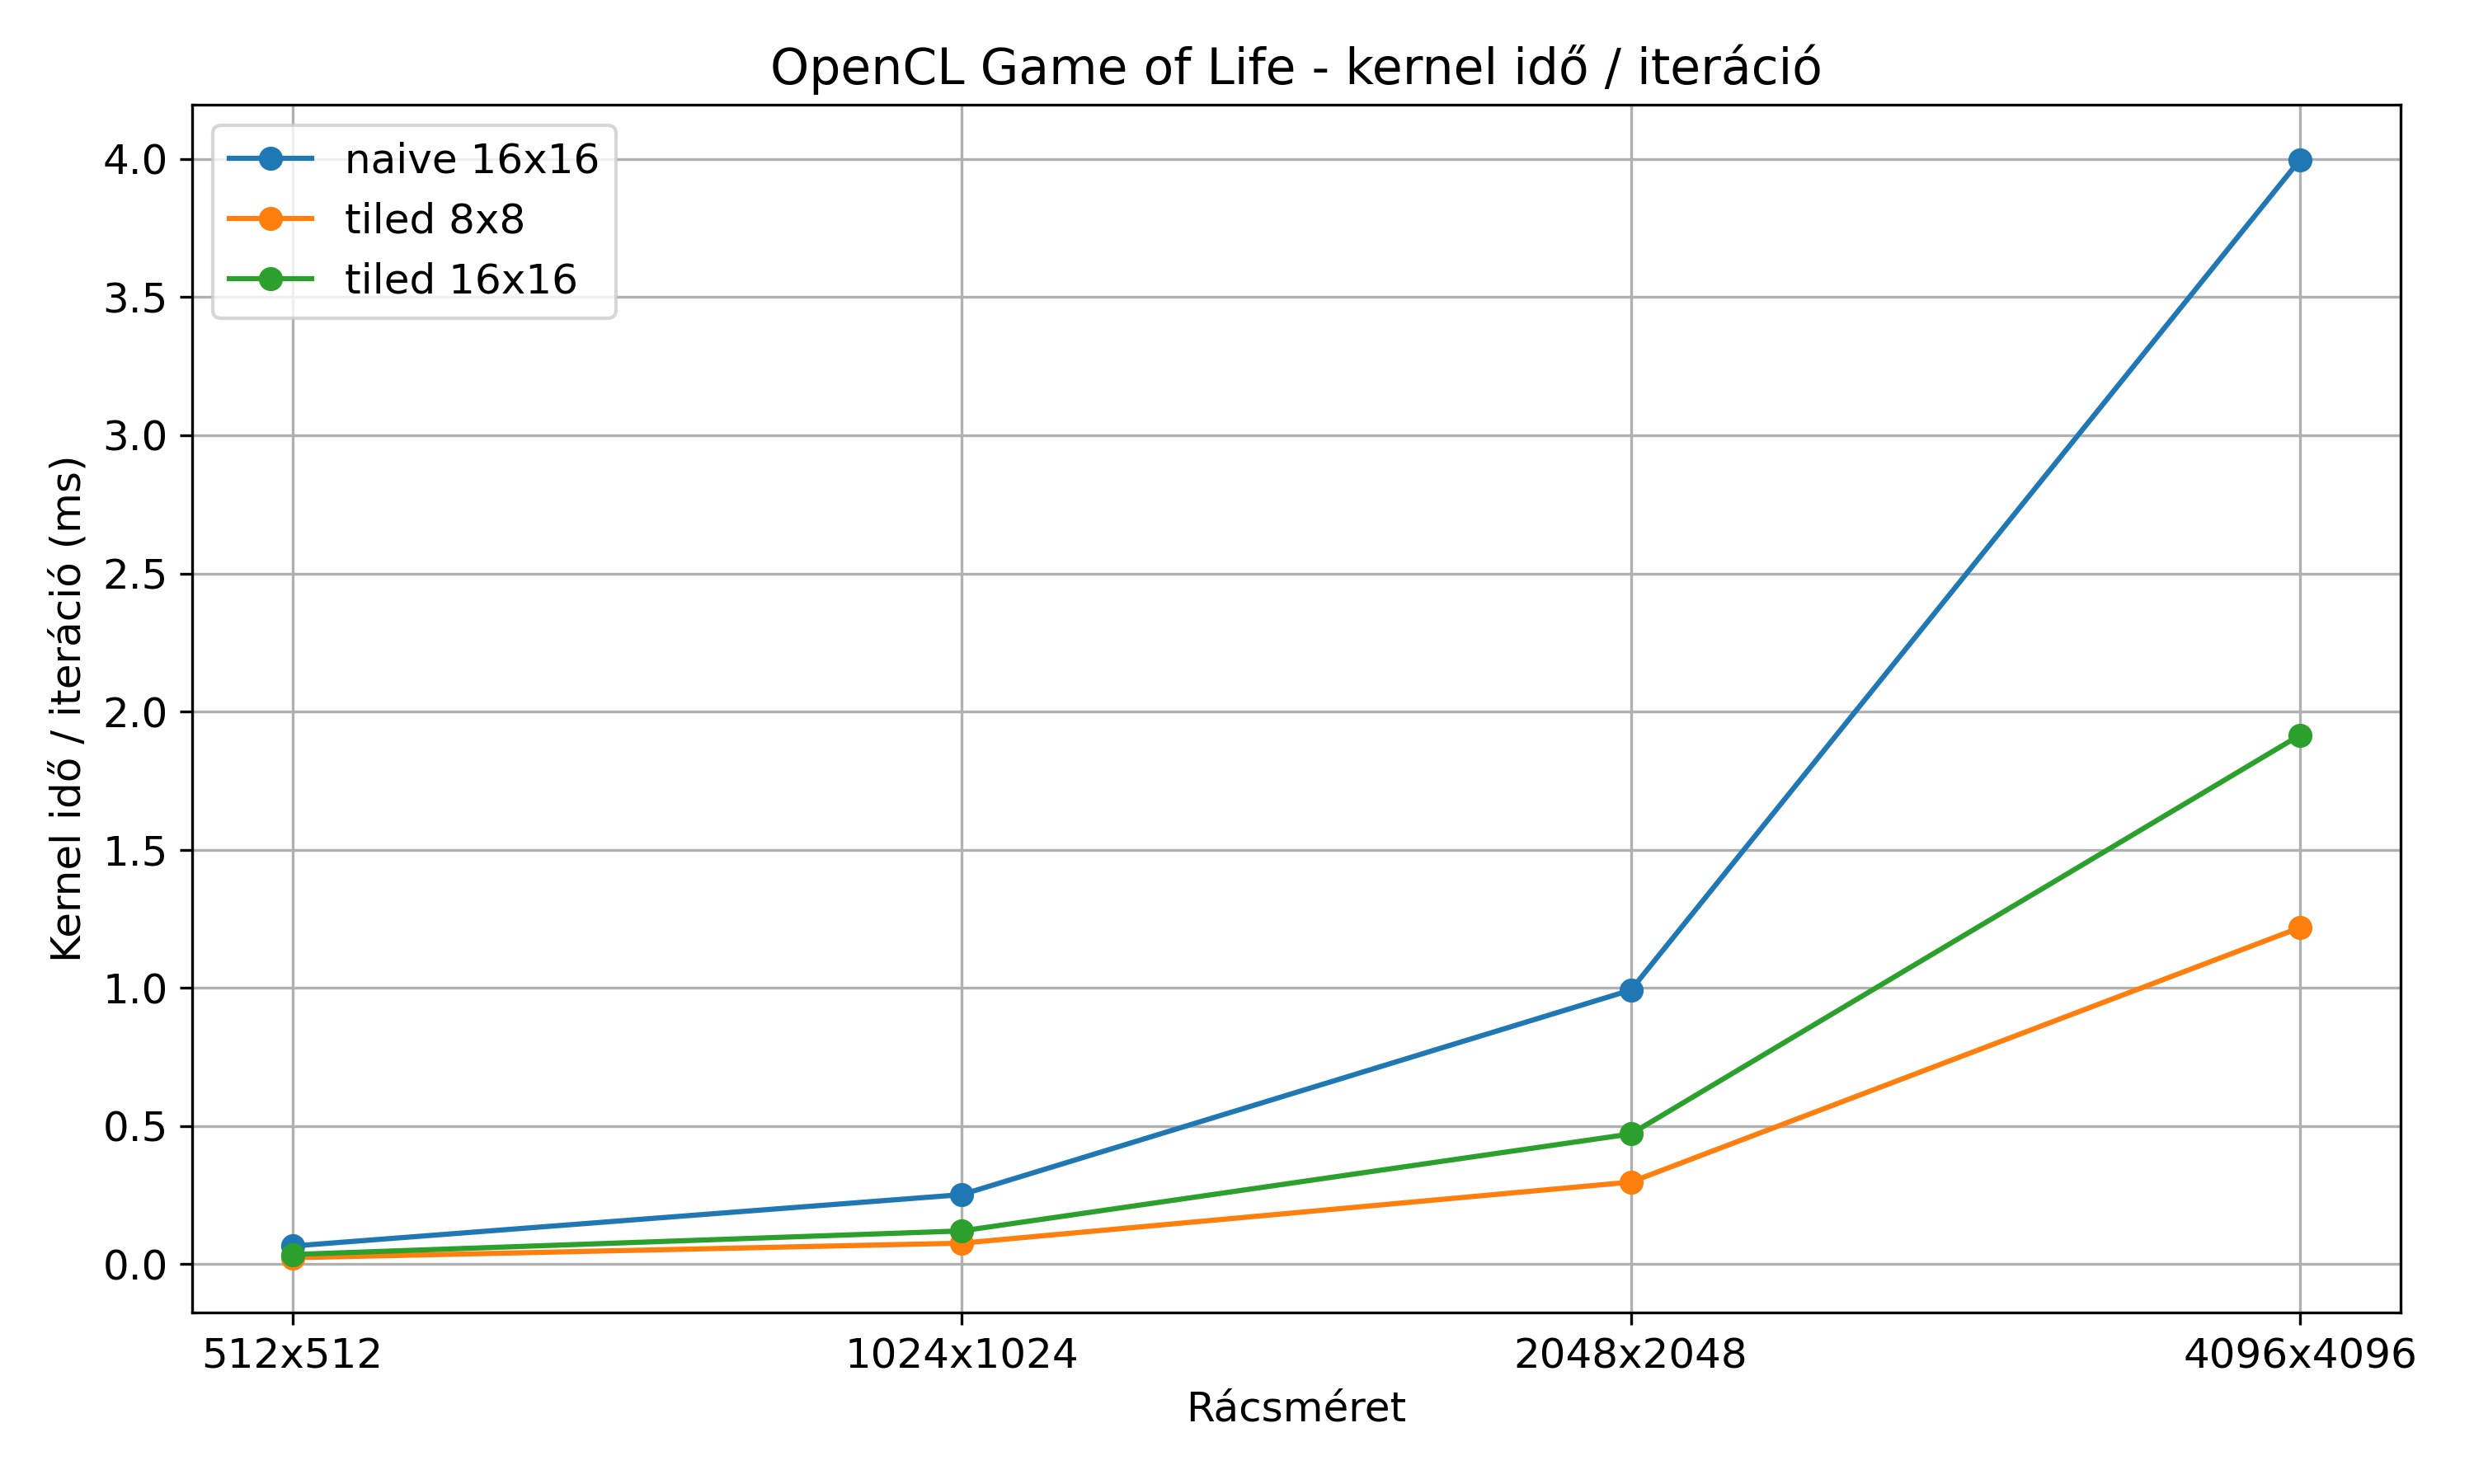
\includegraphics[width=0.9\textwidth]{figures/kernel_per_iter.png}
    \caption{A kernel futási ideje iterációnként különböző rácsméretek esetén.}
    \label{fig:kernel_per_iter}
\end{figure}

A \ref{fig:kernel_per_iter}. ábra jól szemlélteti, hogy a rácsméret növekedésével a kernelidő minden vizsgált konfigurációban nő, ugyanakkor az optimalizált \emph{tiled} megoldások végig kedvezőbb eredményt adnak, mint a referencia-naiv implementáció.

\section{Mérési eredmények}

A fő mérési sorozat eredményei alapján a \emph{tiled} OpenCL megoldás minden vizsgált rácsméret esetén gyorsabbnak bizonyult a naiv implementációnál. Ez egyértelműen azt mutatja, hogy a lokális memória használata hatékonyan csökkenti a globális memóriaelérések költségét, és ez a gyakorlatban is jól mérhető teljesítményjavulást eredményez.

\begin{table}[H]
\centering
\caption{A fő mérési eredmények összefoglalása a \texttt{wrap=0} esetén.}
\label{tab:main_results}
\resizebox{\textwidth}{!}{%
\begin{tabular}{lrrrrr}
\toprule
Rácsméret & Naiv kernelidő (ms) & Tiled 8x8 (ms) & Tiled 16x16 (ms) & 8x8 gyorsulás & 16x16 gyorsulás \\
\midrule
512x512   & 131.17 & 46.37  & 69.86  & 2.83x & 1.88x \\
1024x1024 & 251.60 & 75.93  & 120.34 & 3.31x & 2.09x \\
2048x2048 & 496.07 & 148.52 & 235.65 & 3.34x & 2.11x \\
4096x4096 & 999.47 & 304.57 & 478.78 & 3.28x & 2.09x \\
\bottomrule
\end{tabular}%
}
\end{table}

A \ref{tab:main_results}. táblázat összefoglalja a fő mérési sorozat legfontosabb kernelidő- és gyorsulási eredményeit a \texttt{wrap=0} peremkezelési mód esetén.

A \texttt{512x512} méretű rács esetén a naiv implementáció kernelideje \texttt{131.17 ms} volt, míg a \texttt{tiled 8x8} konfiguráció \texttt{46.37 ms}, a \texttt{tiled 16x16} konfiguráció pedig \texttt{69.86 ms} értéket adott. Ebben az esetben tehát mindkét optimalizált változat gyorsabb volt a referencia-megoldásnál, és a kisebb rácsméreten már a \texttt{tiled 8x8} bizonyult a legjobb választásnak.

A \texttt{1024x1024} méretű rácsnál a különbség még látványosabbá vált. A naiv megoldás \texttt{251.60 ms} kernelidőt mutatott, míg a \texttt{tiled 8x8} változat \texttt{75.93 ms}, a \texttt{tiled 16x16} pedig \texttt{120.34 ms} eredményt adott. Itt a \texttt{tiled 8x8} konfiguráció körülbelül \texttt{3.31}-szeres gyorsulást ért el a naiv verzióhoz képest.

A \texttt{2048x2048} rácsméretnél a naiv implementáció \texttt{496.07 ms}, a \texttt{tiled 8x8} \texttt{148.52 ms}, a \texttt{tiled 16x16} pedig \texttt{235.65 ms} kernelidőt adott. A \texttt{tiled 8x8} konfiguráció ebben az esetben is jelentős előnyt mutatott, és megközelítőleg \texttt{3.34}-szeres gyorsulást biztosított.

A legnagyobb, \texttt{4096x4096} méretű rács esetén a naiv megoldás \texttt{999.47 ms} kernelidőt mutatott, míg a \texttt{tiled 8x8} konfiguráció \texttt{304.57 ms}, a \texttt{tiled 16x16} pedig \texttt{478.78 ms} értéket adott. Ez azt jelenti, hogy a \texttt{tiled 8x8} megoldás a legnagyobb vizsgált méreten is hozzávetőleg \texttt{3.28}-szoros gyorsulást ért el a naiv implementációhoz képest.

Az eredményekből jól látszik, hogy a \emph{tiled} megközelítés minden esetben előnyösebb volt a naiv verziónál, ugyanakkor a két optimalizált konfiguráció között is jelentős különbség mutatkozott. A vizsgált hardveren a \texttt{8x8} méretű \emph{work-group} bizonyult a legjobb választásnak a közepes és nagyobb rácsméretek esetén, míg a \texttt{16x16} méretű \emph{tiled} megoldás ugyan gyorsabb volt a naiv változatnál, de teljesítménye minden nagyobb vizsgált méreten elmaradt a \texttt{8x8} konfigurációétól. Ez azt mutatja, hogy a \emph{work-group} méret megválasztása lényegesen befolyásolja a teljesítményt.

A mért hardverkörnyezetben a \texttt{tiled 8x8} konfiguráció azért is lehetett kedvezőbb a \texttt{tiled 16x16} beállításnál, mert a kisebb \emph{work-group} gyakran rugalmasabban illeszkedik a GPU erőforrásaihoz. A nagyobb csoportméret ugyan elméletileg több adat együttes feldolgozását teszi lehetővé, a gyakorlatban azonban növelheti a lokális memóriaigényt, a regiszterhasználatot és ronthatja az egyidejűleg futtatható \emph{work-groupok} számát. Emiatt előfordulhat, hogy a \texttt{16x16} konfiguráció kisebb erőforrás-kihasználást vagy kedvezőtlenebb ütemezést eredményez, míg a \texttt{8x8} beállítás jobb egyensúlyt ad a lokális memóriahasználat, az ütemezhetőség és a párhuzamosság között. A kapott eredmények alapján a vizsgált GPU-n ez a kompromisszum a \texttt{tiled 8x8} változatnak kedvezett.

\begin{figure}[H]
    \centering
    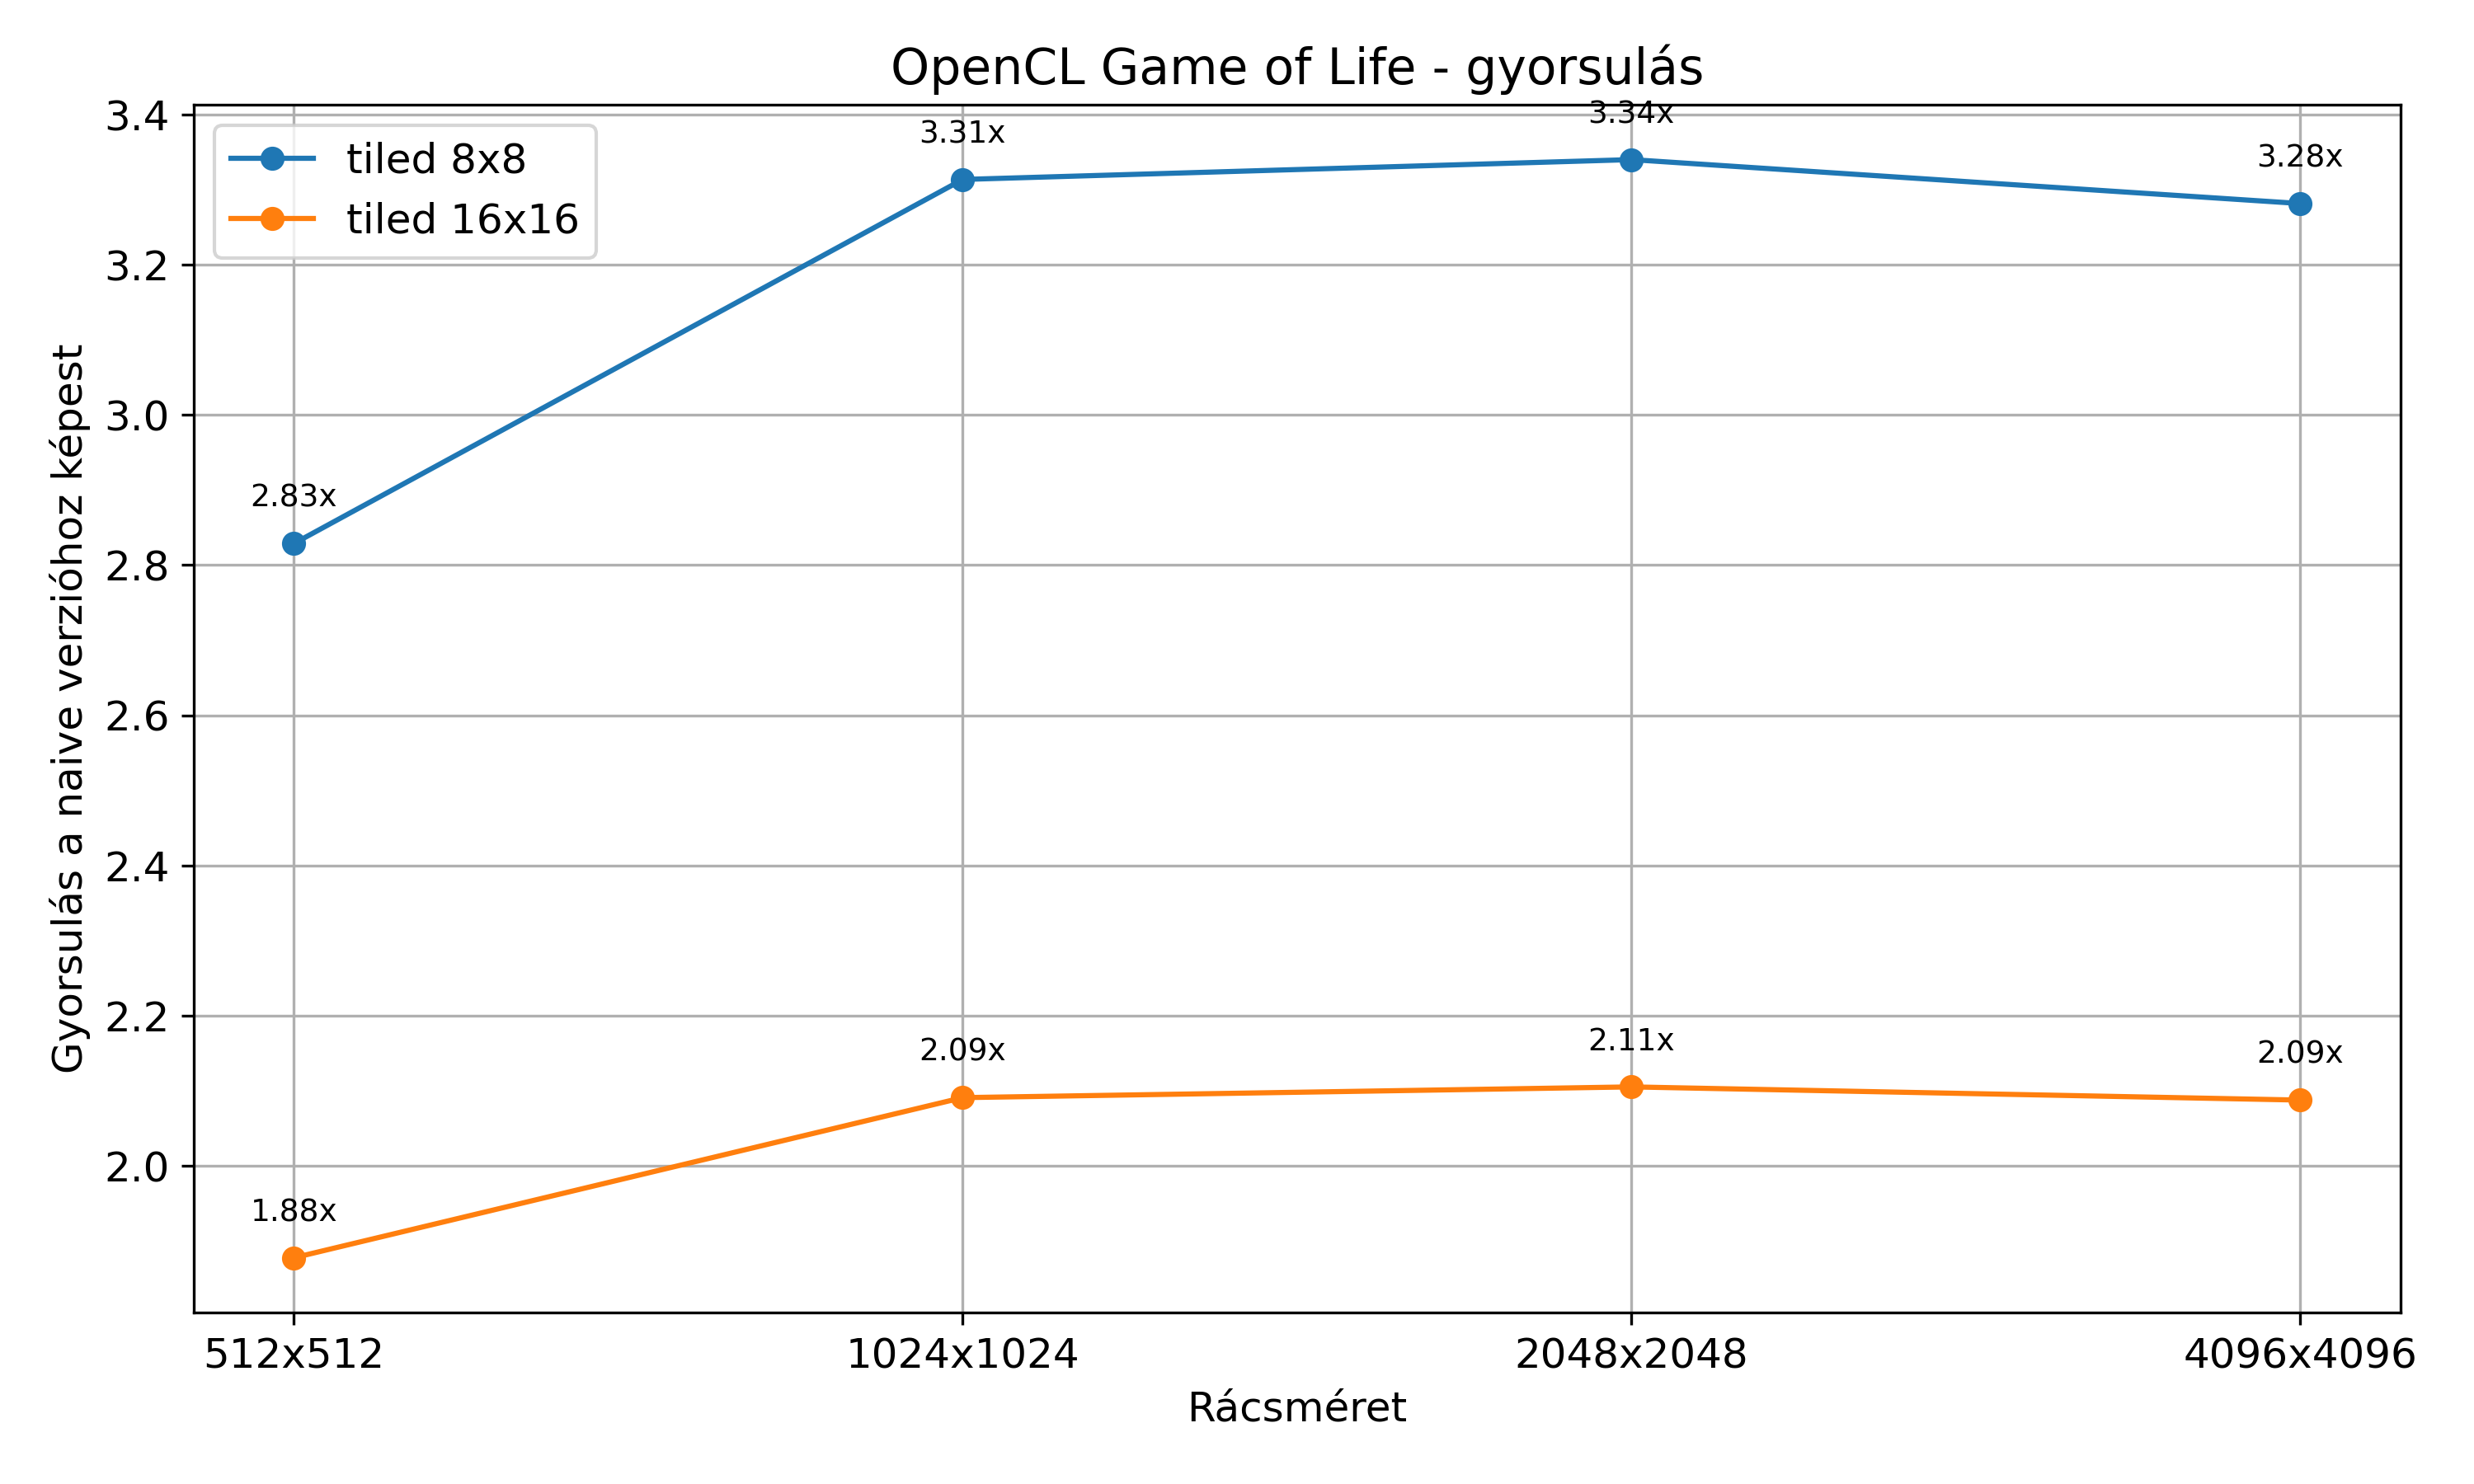
\includegraphics[width=0.9\textwidth]{figures/speedup.png}
    \caption{A \emph{tiled} megoldások gyorsulása a naiv implementációhoz képest.}
    \label{fig:speedup}
\end{figure}

A \ref{fig:speedup}. ábra alapján a \texttt{tiled 8x8} konfiguráció gyorsulása rendre \texttt{2.83x}, \texttt{3.31x}, \texttt{3.34x} és \texttt{3.28x} volt a vizsgált rácsméreteken. A \texttt{tiled 16x16} konfiguráció gyorsulása ezzel szemben \texttt{1.88x}, \texttt{2.09x}, \texttt{2.11x} és \texttt{2.09x} értékeket adott. A gyorsulási görbe jól mutatja, hogy az optimalizált megközelítés különösen nagyobb rácsméretek mellett válik igazán előnyössé.

Az összegzett profilozott végrehajtási idő vizsgálata azt mutatja, hogy a kernelidő dominálja a végrehajtást, míg a host--device és device--host adatmásolások költsége ehhez képest viszonylag kicsi marad. Ez különösen a nagyobb rácsméretek esetén figyelhető meg, ahol az összegzett profilozott végrehajtási idő alakulását döntően a kernel teljesítménye határozza meg.

\begin{figure}[H]
    \centering
    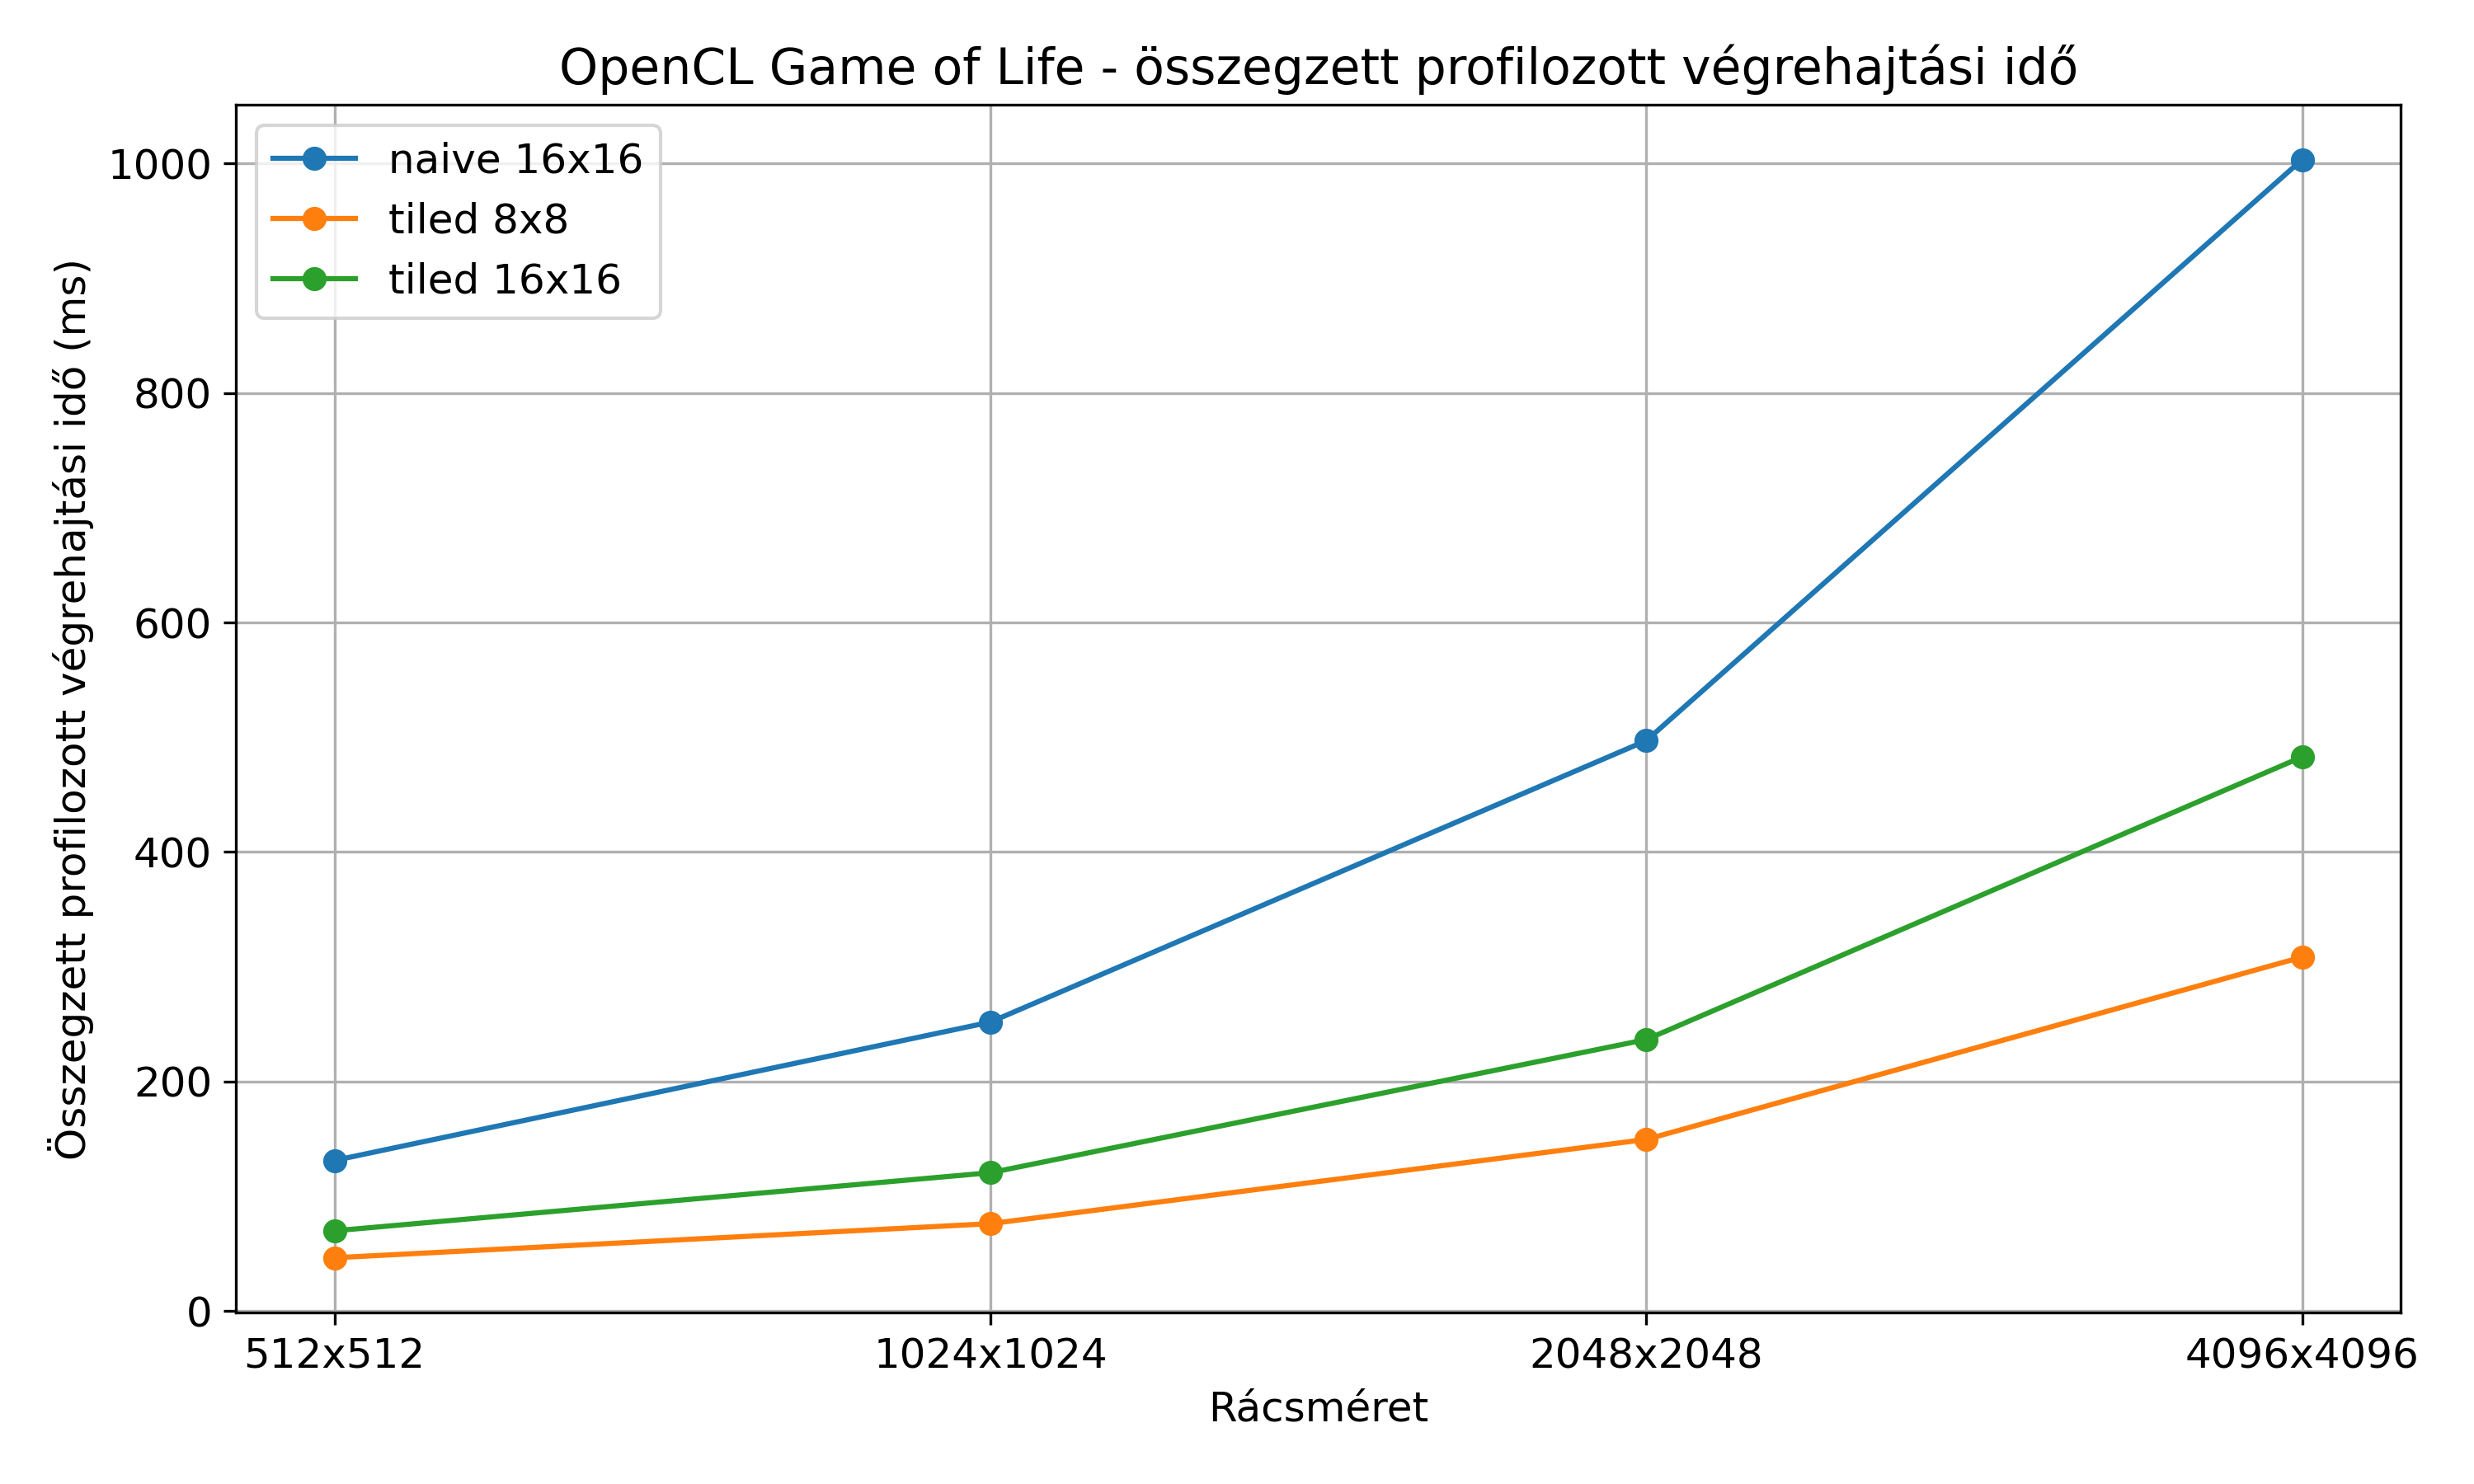
\includegraphics[width=0.9\textwidth]{figures/total_time.png}
    \caption{Az összegzett profilozott végrehajtási idő összehasonlítása a vizsgált implementációk esetén.}
    \label{fig:total_time}
\end{figure}

A \ref{fig:total_time}. ábra szerint az összegzett profilozott végrehajtási idők szintén megerősítik a kernelidőknél tapasztalt sorrendet. A naiv implementáció minden méreten a leglassabb, míg a \texttt{tiled 8x8} konfiguráció adja a legkedvezőbb eredményt. A másolási idők hozzájárulása a teljes végrehajtáshoz a vizsgált esetekben kicsi, ezért a teljesítményjavulás elsődleges forrása valóban a kernel optimalizálásából származik.

A külön elvégzett wrap-összehasonlító mérések azt mutatták, hogy a peremkezelés módja kisebb, de jól mérhető hatással lehet a futási időre. A naiv implementáció esetében a \texttt{wrap=0} és \texttt{wrap=1} közötti különbség viszonylag kicsi maradt: \texttt{1024x1024} méret esetén a \texttt{wrap=1} kismértékben lassabbnak, míg \texttt{2048x2048} méret esetén minimálisan gyorsabbnak bizonyult. Ezzel szemben a \emph{tiled 16x16} konfigurációban a toroidális peremkezelés minden vizsgált esetben lassabb futást eredményezett. \texttt{1024x1024} méret mellett a kernelidő \texttt{119.73 ms}-ról \texttt{129.97 ms}-ra, míg \texttt{2048x2048} méretnél \texttt{251.59 ms}-ról \texttt{254.84 ms}-ra nőtt.

\begin{figure}[H]
    \centering
    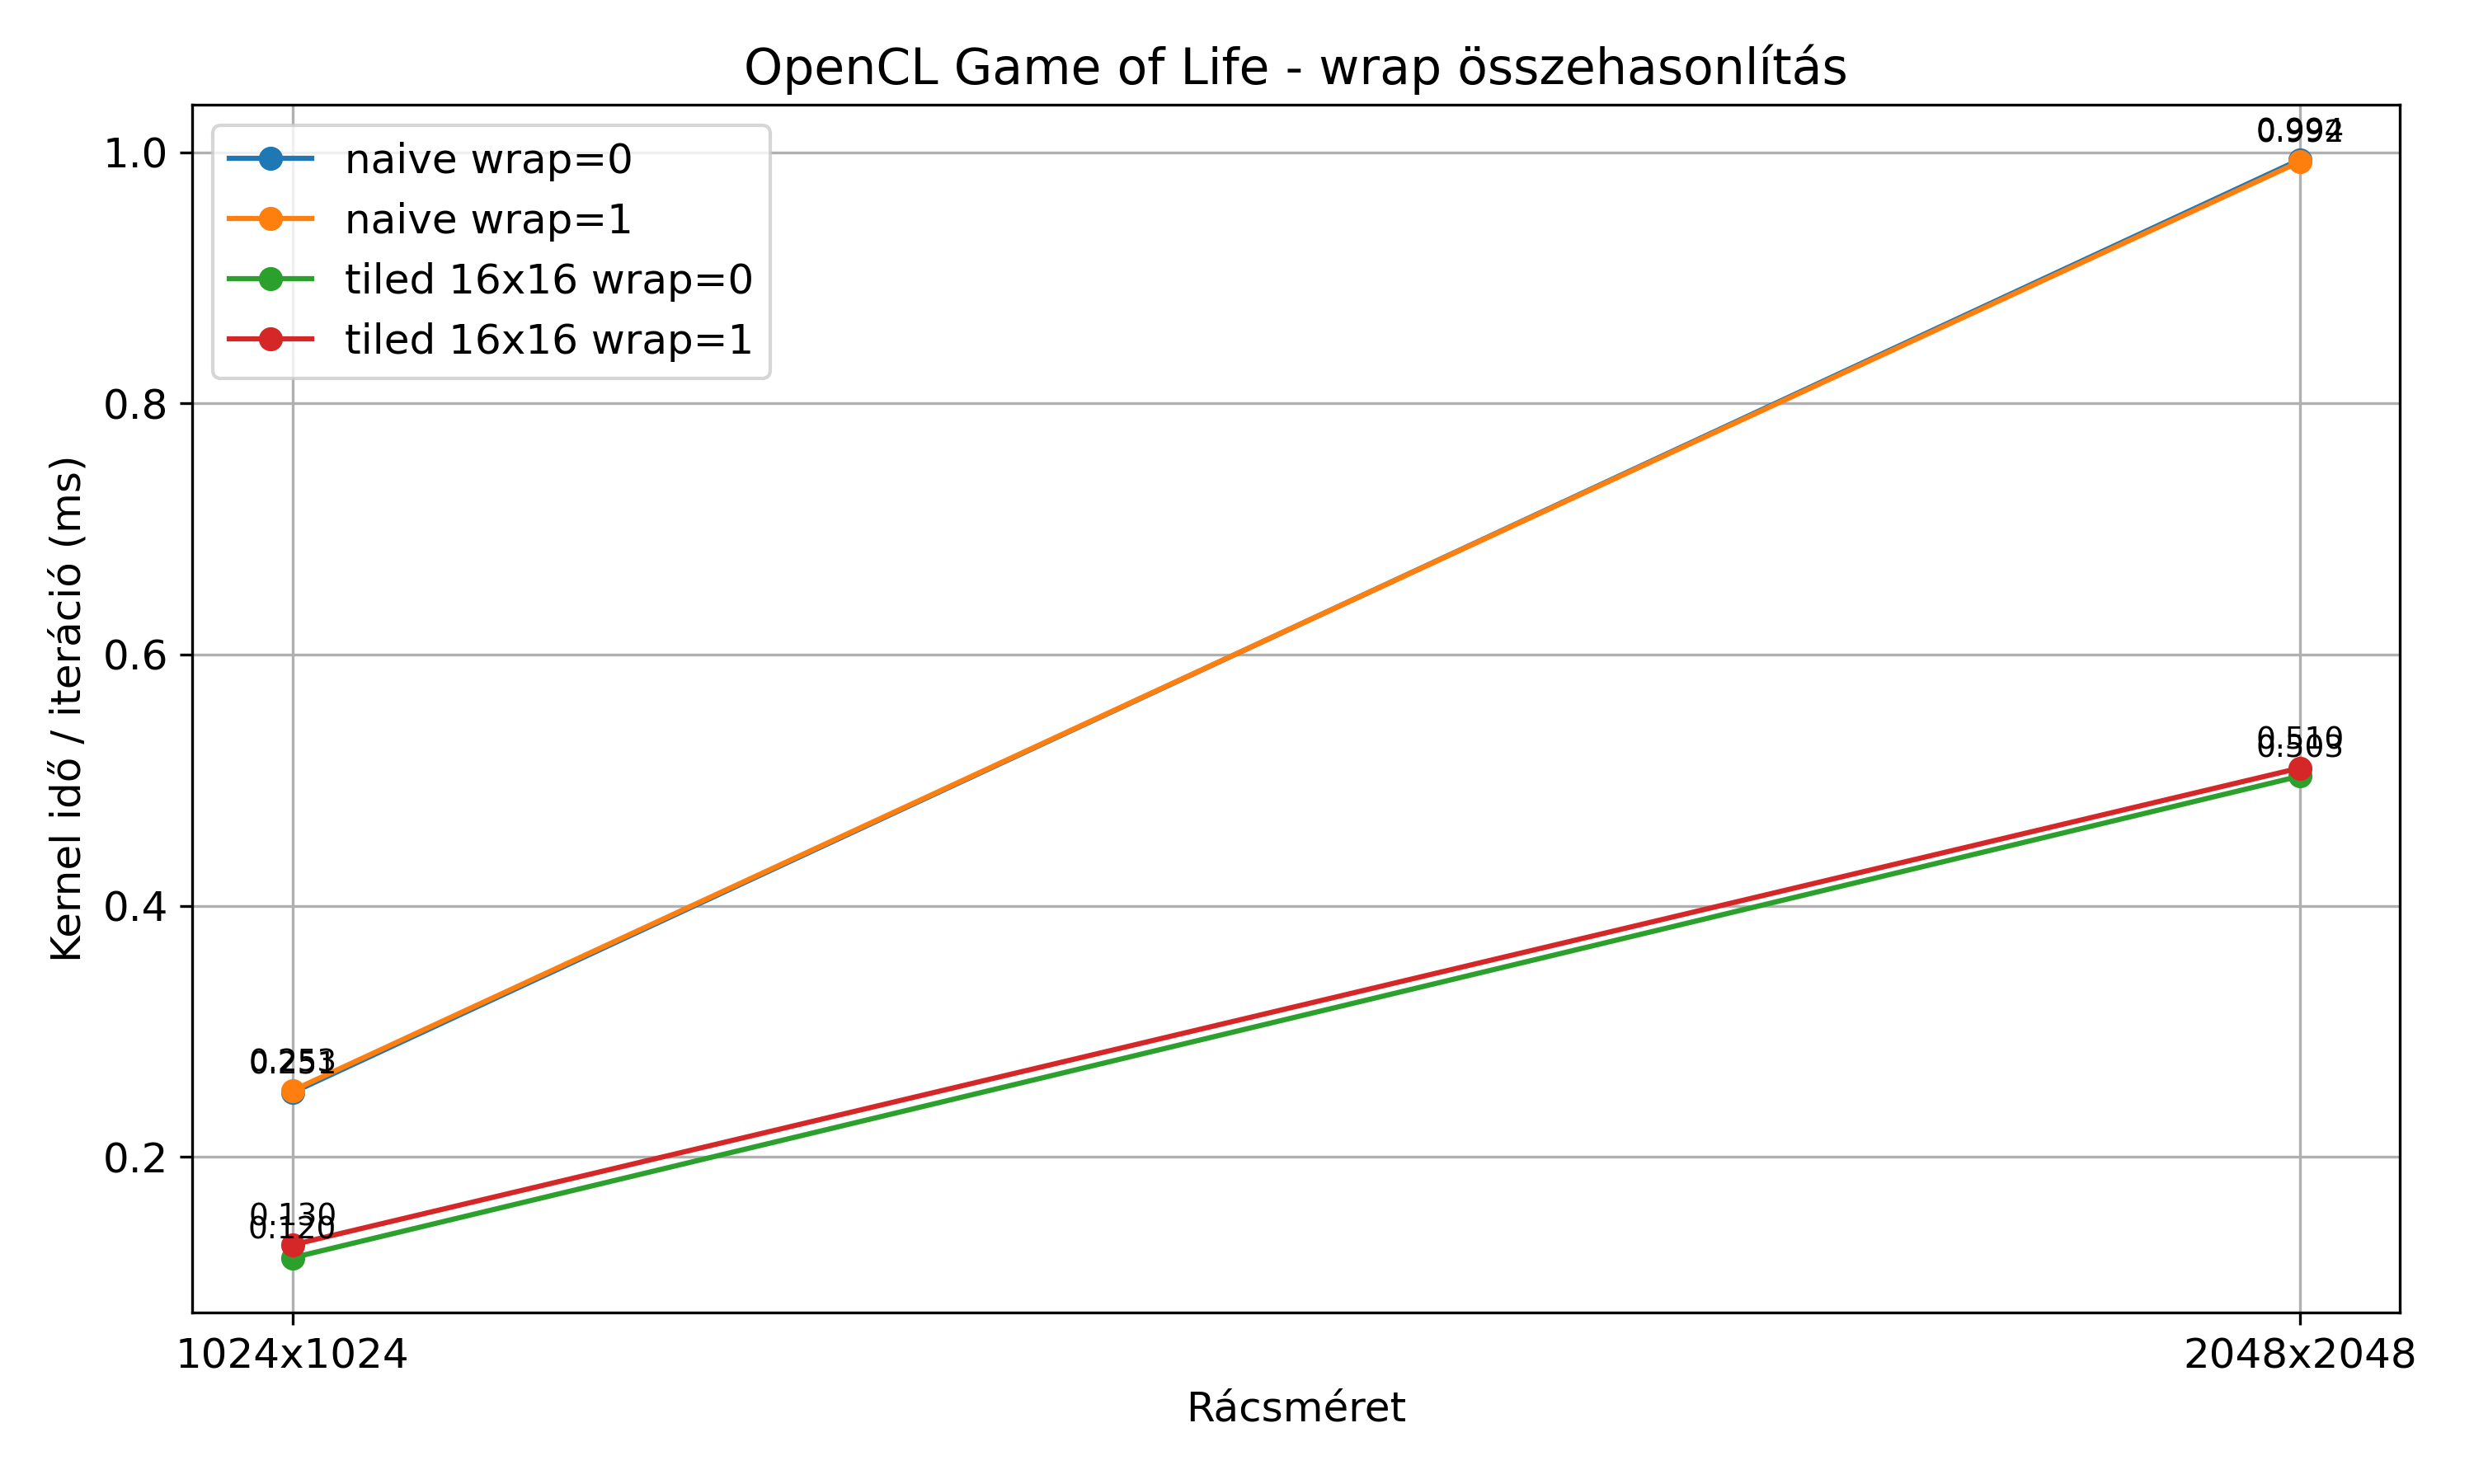
\includegraphics[width=0.9\textwidth]{figures/wrap_kernel_compare.png}
    \caption{A peremkezelés módjának hatása a kernel futási idejére.}
    \label{fig:wrap_compare}
\end{figure}

A \ref{fig:wrap_compare}. ábra alapján megállapítható, hogy a peremkezelés hatása nem domináns tényező, ugyanakkor a \emph{tiled} megoldásban jól láthatóan növeli a futási időt. Ez valószínűleg az összetettebb indexkezelésből és a peremfeltételek kezelésének többletköltségéből adódik.

A mérési eredmények összességében igazolják, hogy a Game of Life OpenCL-alapú megvalósításában a lokális memória használata hatékony optimalizáció, és megfelelő \emph{work-group} méret mellett jelentős gyorsulás érhető el a naiv implementációhoz képest. A vizsgált konfigurációk közül a legtöbb esetben a \texttt{tiled 8x8} megoldás bizonyult a legjobb választásnak, ezért a mért hardverkörnyezetben ez tekinthető a legkedvezőbb beállításnak.

\section{Kiértékelés}

A kapott eredmények alapján egyértelműen megállapítható, hogy a Game of Life OpenCL-alapú megvalósításában a \emph{tiled} megközelítés hatékonyabbnak bizonyult a naiv implementációnál. A különbség minden vizsgált rácsméreten megjelent, és a gyorsulás különösen a nagyobb problémaméretek esetén vált hangsúlyossá. Ez alátámasztja azt a várakozást, hogy a globális memóriaelérések csökkentése és a lokális memória tudatos használata jelentős teljesítményelőnyt eredményezhet.

A naiv és a \emph{tiled} megoldás összehasonlítása jól mutatja az optimalizáció gyakorlati hasznát. A naiv kernel előnye az egyszerűség és az átlátható működés, ugyanakkor minden cella feldolgozása során sok globális memóriaelérést végez. Ezzel szemben a \emph{tiled} megoldás a szomszédsági vizsgálathoz szükséges adatokat először lokális memóriába tölti, így a további hozzáférések gyorsabb memóriaterületről történnek. A mérések azt mutatták, hogy ez a szervezés nem pusztán elméleti optimalizáció, hanem a gyakorlatban is stabilan jobb futási időket eredményezett.

A két \emph{tiled} konfiguráció összevetése szintén fontos tanulságot adott. A vizsgált hardveren a \texttt{8x8} méretű \emph{work-group} bizonyult kedvezőbbnek a \texttt{16x16} beállításnál, különösen a közepes és nagyobb rácsméretek esetén. Ez arra utal, hogy a \emph{work-group} méret megválasztása érzékenyen befolyásolja a teljesítményt, vagyis nem elegendő csupán lokális memóriát használni, hanem annak kihasználását a hardver sajátosságaihoz is érdemes igazítani. A mért konfigurációk alapján a \texttt{tiled 8x8} megoldás adta a legjobb kompromisszumot az erőforrás-kihasználás és a memóriahozzáférések szervezése között.

A rácsméret növekedésével a futási idő minden esetben emelkedett, ami természetes következménye annak, hogy nagyobb probléma esetén több cella állapotát kell minden iterációban újraszámítani. Ugyanakkor az is jól látszott, hogy az optimalizált megoldás előnye nagyobb méreteken sem tűnik el, sőt, inkább hangsúlyosabbá válik. Ez különösen fontos megfigyelés, mert azt mutatja, hogy az alkalmazott optimalizáció nemcsak kis példákon működik jól, hanem nagyobb számítási terhelés mellett is releváns marad.

Az összegzett profilozott végrehajtási idők elemzése alapján a kernel futási ideje dominálja a végrehajtást, míg a host--device és device--host másolások ehhez képest kisebb szerepet játszanak. Ez azért lényeges, mert így a teljesítménykülönbség valóban a kernelmegoldások közötti eltérésből fakad, nem pedig valamilyen külső, mérésen kívüli tényezőből. Másképpen fogalmazva: a gyorsulás fő forrása a számítási mag jobb megszervezése volt.

A wrap-összehasonlító mérések kiegészítő eredményként azt mutatták, hogy a peremkezelés módja ugyan nem a legmeghatározóbb tényező, de mérhető hatással van a futási időre. A naiv implementáció esetében a különbség kicsi maradt, míg a \emph{tiled 16x16} konfigurációban a toroidális peremkezelés általában lassabb futást eredményezett. Ez arra utal, hogy az összetettebb indexkezelésnek és a peremfeltételek kezelésének van ugyan többletköltsége, de ez a hatás még mindig kisebb jelentőségű, mint maga a memóriahasználati stratégia.

Összességében a mérések azt igazolták, hogy a projektben alkalmazott optimalizációk nemcsak elméletben indokolhatók, hanem a gyakorlatban is egyértelműen jobb eredményt adnak. A beadandó legfontosabb tanulsága az, hogy OpenCL környezetben a teljesítményt jelentősen befolyásolja a memóriaelérések szervezése, a \emph{work-group} méret megválasztása, valamint az, hogy a feladat mennyire illeszkedik az adatpárhuzamos végrehajtási modellhez.

\section{Összegzés}

A beadandó során sikerült elkészíteni a Conway-féle Game of Life OpenCL-alapú, párhuzamos megvalósítását. A fejlesztés eredményeként egy olyan program jött létre, amely képes különböző méretű rácsok több iteráción keresztüli feldolgozására, támogatja a kétféle peremkezelési módot, parancssori paraméterekkel vezérelhető, valamint alkalmas teljesítménymérések elvégzésére és azok CSV formátumú rögzítésére.

A projekt során két különböző kernelváltozat készült. A naiv implementáció egyszerű és jól áttekinthető referencia-megoldást adott, míg a lokális memóriát használó \emph{tiled} megközelítés lehetővé tette a teljesítmény javítását. A mérések alapján egyértelműen kimutatható volt, hogy a \emph{tiled} megoldás minden vizsgált méreten gyorsabb a naiv verziónál, és a tesztelt konfigurációk közül a \texttt{tiled 8x8} bizonyult a legkedvezőbb választásnak.

A beadandó egyik legfontosabb tanulsága az volt, hogy a GPU-alapú párhuzamos feldolgozásban nem elegendő pusztán a feladat párhuzamosíthatósága. Legalább ennyire meghatározó a memóriahasználat módja, az adatok elrendezése, valamint a \emph{work-group} méret helyes megválasztása is. A kapott eredmények jól mutatták, hogy megfelelő optimalizációval jelentős gyorsulás érhető el ugyanazon algoritmus esetén.

A projekt további fejlesztési lehetőségeket is kínál. Érdekes irány lehetne további \emph{work-group} méretek vizsgálata, nem négyzetes rácsméretek tesztelése, illetve a CPU- és GPU-változat részletesebb összehasonlítása. A program fejlesztése során CPU referenciaalapú validációs lehetőség is bekerült, amely lehetővé teszi a GPU eredményeinek összehasonlítását egy CPU referenciaimplementációval. Ez különösen hasznos a helyes működés ellenőrzésére kisebb vagy tesztcélú futtatások esetén. További lehetőséget jelenthetne a program vizualizációval való kiegészítése is, amely szemléletesebbé tenné az egyes generációk alakulását.

Összességében a beadandó elérte a kitűzött célját: bemutatta, hogy a Conway-féle Game of Life hatékonyan megvalósítható OpenCL segítségével, és megfelelő optimalizáció alkalmazásával a naiv megközelítéshez képest számottevő teljesítményjavulás érhető el. A projekt így nemcsak működő programot, hanem jól értelmezhető mérési eredményeket és gyakorlati tapasztalatokat is adott a párhuzamos programozás és a GPU-s végrehajtás területén.

\end{document}